\documentclass[11pt,a4paper]{article}
\usepackage[margin=1in]{geometry}
\usepackage{amsmath,amssymb,amsthm}
\usepackage{mathtools}
\usepackage{enumitem}
\usepackage{xcolor}
\usepackage{tcolorbox}
\usepackage{tikz}
\usetikzlibrary{arrows.meta,decorations.markings}

% Custom commands for XYZ methodology
\newcommand{\stage}[1]{\textbf{\textcolor{blue}{#1}}}
\newcommand{\critical}[1]{\textbf{\textcolor{red}{#1}}}

\title{Exercise Sheet 1: Question 2\\
Finite Time Blow Up\\
Methods of Applied Mathematics [SEMT30006]}
\author{Complete Solutions with XYZ Methodology}
\date{}

\begin{document}

\maketitle

\section*{Problem Statement}

Solve the initial value problem
\begin{equation}
\dot{x} = ax^2
\end{equation}
with $x(0) = x_0$.

\begin{enumerate}[label=(\alph*)]
    \item Does this have solutions, are they unique, and where do they exist?
    \item Solve the equations for $x(t)$ in terms of $a$ and $x_0$.
    \item Despite your answer to (a), show that something 'goes wrong' at time $t = \frac{1}{ax_0}$, and describe what happens there. This is known as finite time blow up.
    \item Sketch a solution for $a = 1$ and $x_0 = 0.2$.
\end{enumerate}

\vspace{0.5cm}

\critical{CONTEXT FROM COURSE:} This problem explores the boundaries of existence and uniqueness theorems (lecture notes pages 14-18). We will see that even though solutions exist and are unique \textit{locally}, they may not exist for all time $t \in \mathbb{R}$. This is a fundamental phenomenon in nonlinear ODEs called \textbf{finite time blow up}.

\newpage

\section{Problem 2(a): Existence, Uniqueness, and Domain of Solutions}

\subsection*{Step 1: State the Relevant Theorems}

\begin{itemize}[leftmargin=*]
\item \stage{STAGE X (What we need):}
For the initial value problem $\dot{x} = f(x, t)$ with $x(t_0) = x_0$, we need to check conditions for:
\begin{enumerate}
    \item \textbf{Existence:} Does a solution exist?
    \item \textbf{Uniqueness:} Is the solution unique?
    \item \textbf{Domain:} For what values of $t$ does the solution exist?
\end{enumerate}

\item \stage{STAGE Y (Relevant theorems):}
From lecture notes (pages 14-18), the key result is:

\textbf{Picard-Lindelöf Theorem (Existence and Uniqueness):}
If $f(x, t)$ is:
\begin{itemize}
    \item Continuous in both $x$ and $t$ in some region $R$ containing $(x_0, t_0)$
    \item Lipschitz continuous in $x$ (i.e., $|f(x_1, t) - f(x_2, t)| \leq L|x_1 - x_2|$ for some constant $L$)
\end{itemize}
then there exists a unique solution in some interval $|t - t_0| < \delta$.

The theorem guarantees \textbf{local} existence and uniqueness but not necessarily \textbf{global} (for all $t$).

\item \stage{STAGE Z (Our specific problem):}
For $\dot{x} = ax^2$, we have $f(x, t) = ax^2$. We need to check:
\begin{enumerate}
    \item Continuity of $f$
    \item Lipschitz continuity in $x$
\end{enumerate}
\end{itemize}

\subsection*{Step 2: Check Continuity}

\begin{itemize}[leftmargin=*]
\item \stage{STAGE X (Examining $f(x, t) = ax^2$):}
The function $f(x, t) = ax^2$ is:
\begin{itemize}
    \item A polynomial in $x$
    \item Independent of $t$ (autonomous system)
    \item Continuous everywhere in $\mathbb{R} \times \mathbb{R}$
\end{itemize}

\item \stage{STAGE Y (Why this matters):}
Polynomial functions are continuous everywhere. Since $f$ does not depend on $t$, continuity in $t$ is trivial. Therefore, the first condition of the Picard-Lindelöf theorem is satisfied.

\item \stage{STAGE Z (Conclusion):}
$\checkmark$ \textbf{Continuity condition satisfied} for all $(x, t) \in \mathbb{R} \times \mathbb{R}$.
\end{itemize}

\subsection*{Step 3: Check Lipschitz Continuity}

\begin{itemize}[leftmargin=*]
\item \stage{STAGE X (Lipschitz condition definition):}
A function $f(x)$ is Lipschitz continuous on an interval $I$ if there exists a constant $L \geq 0$ such that:
\begin{equation}
|f(x_1) - f(x_2)| \leq L|x_1 - x_2| \quad \forall x_1, x_2 \in I
\end{equation}

\item \stage{STAGE Y (Testing $f(x) = ax^2$):}
Consider the difference:
\begin{align}
|f(x_1) - f(x_2)| &= |ax_1^2 - ax_2^2| \\
&= |a||x_1^2 - x_2^2| \\
&= |a||x_1 + x_2||x_1 - x_2|
\end{align}

For Lipschitz continuity, we need:
\begin{equation}
|a||x_1 + x_2||x_1 - x_2| \leq L|x_1 - x_2|
\end{equation}

This simplifies to:
\begin{equation}
|a||x_1 + x_2| \leq L
\end{equation}

\textbf{Problem:} If $x_1$ or $x_2$ can be arbitrarily large, then $|x_1 + x_2|$ can be arbitrarily large, so no single constant $L$ works for all $x_1, x_2 \in \mathbb{R}$.

\item \stage{STAGE Z (Local vs. Global Lipschitz):}
\begin{itemize}
    \item $f(x) = ax^2$ is \textbf{NOT globally Lipschitz} on $\mathbb{R}$
    \item $f(x) = ax^2$ \textbf{IS locally Lipschitz} on any bounded interval $[x_0 - \delta, x_0 + \delta]$
\end{itemize}

On a bounded interval where $|x| \leq M$, we can take $L = 2|a|M$, and Lipschitz continuity holds.
\end{itemize}

\subsection*{Step 4: Apply Existence and Uniqueness Theory}

\begin{itemize}[leftmargin=*]
\item \stage{STAGE X (What the theorem tells us):}
Since $f(x) = ax^2$ is:
\begin{itemize}
    \item Continuous everywhere
    \item Locally Lipschitz continuous near any point $x_0$
\end{itemize}

The Picard-Lindelöf theorem guarantees:
\begin{equation}
\text{A unique solution exists \textbf{locally} near } t = 0
\end{equation}

\item \stage{STAGE Y (What "locally" means):}
There exists some time interval $(-\delta, \delta)$ around $t = 0$ on which a unique solution $x(t)$ exists passing through $(0, x_0)$.

However, the theorem does \textbf{NOT} guarantee:
\begin{itemize}
    \item The solution exists for all $t \geq 0$
    \item The solution exists for all $t \in \mathbb{R}$
\end{itemize}

\item \stage{STAGE Z (The question of global existence):}
Whether the solution exists for all time depends on the behavior of the solution itself. We'll need to solve explicitly to determine this.
\end{itemize}

\subsection*{Step 5: Additional Analysis Using the Derivative}

\begin{itemize}[leftmargin=*]
\item \stage{STAGE X (Alternative Lipschitz check):}
Another way to check local Lipschitz continuity is via the derivative. If $\frac{\partial f}{\partial x}$ is bounded on an interval, then $f$ is Lipschitz on that interval.

\item \stage{STAGE Y (Computing the derivative):}
\begin{equation}
\frac{\partial f}{\partial x} = \frac{\partial}{\partial x}(ax^2) = 2ax
\end{equation}

On any bounded interval $|x| \leq M$:
\begin{equation}
\left|\frac{\partial f}{\partial x}\right| = |2ax| \leq 2|a|M
\end{equation}

So the Lipschitz constant is $L = 2|a|M$ on $[-M, M]$.

\item \stage{STAGE Z (Confirms local Lipschitz):}
This confirms that $f(x) = ax^2$ is locally Lipschitz, supporting our conclusion from Step 3.
\end{itemize}

\subsection*{Answer to Problem 2(a)}

\begin{tcolorbox}[colback=blue!5!white,colframe=blue!75!black,title=\textbf{Solution to 2(a)}]

\textbf{Existence:} Yes, a solution exists locally near $t = 0$.

\textbf{Uniqueness:} Yes, the solution is unique locally near $t = 0$.

\textbf{Domain of existence:}
\begin{itemize}
    \item The Picard-Lindelöf theorem guarantees existence and uniqueness in some interval $|t| < \delta$ for some $\delta > 0$
    \item The solution exists locally but NOT necessarily globally (for all $t \in \mathbb{R}$)
    \item The actual domain depends on the parameters $a$ and $x_0$, which we'll determine by solving explicitly
\end{itemize}

\textbf{Mathematical justification:}
\begin{itemize}
    \item $f(x, t) = ax^2$ is continuous everywhere $\checkmark$
    \item $f(x, t) = ax^2$ is locally Lipschitz continuous near any $x_0$ $\checkmark$
    \item Therefore, by Picard-Lindelöf: local existence and uniqueness are guaranteed
\end{itemize}

\textbf{Key insight:} Local Lipschitz (not global) means solutions exist and are unique near the initial condition, but may "escape to infinity" in finite time.
\end{tcolorbox}

\critical{IMPORTANT:} The lack of global Lipschitz continuity is a warning sign that solutions might not exist for all time. This is exactly what we'll see in parts (b) and (c).

\newpage

\section{Problem 2(b): Explicit Solution}

\subsection*{Step 1: Identify the Type of ODE}

\begin{itemize}[leftmargin=*]
\item \stage{STAGE X (What we have):}
The ODE $\dot{x} = ax^2$ with $x(0) = x_0$ is:
\begin{itemize}
    \item First-order
    \item Autonomous (no explicit $t$ dependence)
    \item Separable (can separate $x$ and $t$ terms)
    \item Nonlinear (quadratic in $x$)
\end{itemize}

\item \stage{STAGE Y (Why separation of variables works):}
We can rewrite as:
\begin{equation}
\frac{dx}{dt} = ax^2 \quad \Rightarrow \quad \frac{dx}{x^2} = a \, dt
\end{equation}

This separates the variables: all $x$ terms on the left, all $t$ terms on the right.

\item \stage{STAGE Z (Strategy):}
Integrate both sides and solve for $x(t)$ using the initial condition.
\end{itemize}

\subsection*{Step 2: Separate Variables and Integrate}

\begin{itemize}[leftmargin=*]
\item \stage{STAGE X (Separation):}
Starting from $\dot{x} = ax^2$, separate:
\begin{equation}
\frac{dx}{x^2} = a \, dt
\end{equation}

\critical{IMPORTANT:} This is valid only when $x \neq 0$. We'll handle the special case $x = 0$ separately.

\item \stage{STAGE Y (Integration):}
Integrate both sides:
\begin{equation}
\int \frac{dx}{x^2} = \int a \, dt
\end{equation}

The left side:
\begin{equation}
\int \frac{dx}{x^2} = \int x^{-2} \, dx = \frac{x^{-1}}{-1} = -\frac{1}{x}
\end{equation}

The right side:
\begin{equation}
\int a \, dt = at + C
\end{equation}

\item \stage{STAGE Z (Combining):}
\begin{equation}
-\frac{1}{x} = at + C
\end{equation}

where $C$ is the constant of integration to be determined from initial conditions.
\end{itemize}

\subsection*{Step 3: Apply Initial Condition}

\begin{itemize}[leftmargin=*]
\item \stage{STAGE X (Using $x(0) = x_0$):}
At $t = 0$:
\begin{equation}
-\frac{1}{x(0)} = a(0) + C \quad \Rightarrow \quad -\frac{1}{x_0} = C
\end{equation}

\item \stage{STAGE Y (Substituting back):}
\begin{equation}
-\frac{1}{x} = at - \frac{1}{x_0}
\end{equation}

\item \stage{STAGE Z (Rearranging):}
\begin{equation}
-\frac{1}{x} = at - \frac{1}{x_0} = \frac{ax_0 t - 1}{x_0}
\end{equation}

Therefore:
\begin{equation}
\frac{1}{x} = \frac{1 - ax_0 t}{x_0}
\end{equation}
\end{itemize}

\subsection*{Step 4: Solve for $x(t)$}

\begin{itemize}[leftmargin=*]
\item \stage{STAGE X (Inverting):}
From $\frac{1}{x} = \frac{1 - ax_0 t}{x_0}$:
\begin{equation}
x(t) = \frac{x_0}{1 - ax_0 t}
\end{equation}

\item \stage{STAGE Y (Verification):}
Let's verify this satisfies the ODE. Compute $\dot{x}$:
\begin{align}
x(t) &= \frac{x_0}{1 - ax_0 t} = x_0(1 - ax_0 t)^{-1} \\
\dot{x} &= x_0 \cdot (-1)(1 - ax_0 t)^{-2} \cdot (-ax_0) \\
&= \frac{ax_0^2}{(1 - ax_0 t)^2}
\end{align}

Check if $\dot{x} = ax^2$:
\begin{equation}
ax^2 = a\left(\frac{x_0}{1 - ax_0 t}\right)^2 = \frac{ax_0^2}{(1 - ax_0 t)^2} = \dot{x} \quad \checkmark
\end{equation}

Check initial condition:
\begin{equation}
x(0) = \frac{x_0}{1 - 0} = x_0 \quad \checkmark
\end{equation}

\item \stage{STAGE Z (Solution confirmed):}
The solution $x(t) = \frac{x_0}{1 - ax_0 t}$ satisfies both the ODE and initial condition.
\end{itemize}

\subsection*{Step 5: Handle Special Cases}

\begin{itemize}[leftmargin=*]
\item \stage{STAGE X (Case 1: $x_0 = 0$):}
If $x_0 = 0$, then the initial condition is $x(0) = 0$.

The ODE becomes $\dot{x} = ax^2$. The constant solution $x(t) = 0$ satisfies:
\begin{itemize}
    \item $\dot{x} = 0$
    \item $ax^2 = a \cdot 0^2 = 0$
    \item So $\dot{x} = ax^2$ ✓
\end{itemize}

By uniqueness, $x(t) \equiv 0$ is the unique solution when $x_0 = 0$.

\item \stage{STAGE Y (Case 2: $a = 0$):}
If $a = 0$, the ODE becomes $\dot{x} = 0$, which means $x$ is constant:
\begin{equation}
x(t) = x_0 \quad \text{for all } t
\end{equation}

This agrees with our formula: $x(t) = \frac{x_0}{1 - 0} = x_0$ ✓

\item \stage{STAGE Z (General case):}
For $a \neq 0$ and $x_0 \neq 0$, the solution is:
\begin{equation}
x(t) = \frac{x_0}{1 - ax_0 t}
\end{equation}
\end{itemize}

\subsection*{Answer to Problem 2(b)}

\begin{tcolorbox}[colback=blue!5!white,colframe=blue!75!black,title=\textbf{Solution to 2(b)}]

\textbf{Explicit solution:}
\begin{equation}
\boxed{x(t) = \frac{x_0}{1 - ax_0 t}}
\end{equation}

\textbf{Valid for:} $t \neq \frac{1}{ax_0}$ (assuming $ax_0 \neq 0$)

\textbf{Special cases:}
\begin{itemize}
    \item If $x_0 = 0$: $x(t) \equiv 0$ for all $t$
    \item If $a = 0$: $x(t) = x_0$ for all $t$
    \item If $ax_0 = 0$: solution exists for all $t \in \mathbb{R}$
\end{itemize}

\textbf{Derivation method:} Separation of variables
\begin{equation}
\frac{dx}{x^2} = a \, dt \quad \Rightarrow \quad -\frac{1}{x} = at + C \quad \Rightarrow \quad x = \frac{x_0}{1 - ax_0 t}
\end{equation}
\end{tcolorbox}

\critical{WARNING:} Notice the denominator $1 - ax_0 t$. This becomes zero at $t = \frac{1}{ax_0}$, suggesting something unusual happens at that time!

\newpage

\section{Problem 2(c): Finite Time Blow Up}

\subsection*{Step 1: Identify the Critical Time}

\begin{itemize}[leftmargin=*]
\item \stage{STAGE X (What we have):}
The solution is $x(t) = \frac{x_0}{1 - ax_0 t}$.

The denominator vanishes when:
\begin{equation}
1 - ax_0 t = 0 \quad \Rightarrow \quad t^* = \frac{1}{ax_0}
\end{equation}

(assuming $ax_0 \neq 0$)

\item \stage{STAGE Y (Why this is problematic):}
At $t = t^* = \frac{1}{ax_0}$:
\begin{equation}
x(t^*) = \frac{x_0}{1 - ax_0 \cdot \frac{1}{ax_0}} = \frac{x_0}{1 - 1} = \frac{x_0}{0}
\end{equation}

Division by zero! The solution becomes undefined.

\item \stage{STAGE Z (Different regimes):}
We need to consider different signs of $ax_0$:
\begin{itemize}
    \item If $ax_0 > 0$: $t^* = \frac{1}{ax_0} > 0$ (blow up in forward time)
    \item If $ax_0 < 0$: $t^* = \frac{1}{ax_0} < 0$ (blow up in backward time)
\end{itemize}
\end{itemize}

\subsection*{Step 2: Analyze Behavior as $t \to t^*$ (Case: $ax_0 > 0$)}

\begin{itemize}[leftmargin=*]
\item \stage{STAGE X (Approaching from the left, $t \to t^*-$):}
Consider $t$ slightly less than $t^* = \frac{1}{ax_0}$. Write $t = t^* - \epsilon$ where $\epsilon > 0$ is small:
\begin{align}
1 - ax_0 t &= 1 - ax_0(t^* - \epsilon) \\
&= 1 - ax_0 t^* + ax_0\epsilon \\
&= 1 - 1 + ax_0\epsilon \\
&= ax_0\epsilon
\end{align}

\item \stage{STAGE Y (Behavior of $x(t)$):}
\begin{equation}
x(t) = \frac{x_0}{ax_0\epsilon} = \frac{1}{a\epsilon} \to +\infty \quad \text{as } \epsilon \to 0^+
\end{equation}

Since $ax_0 > 0$, we have $a$ and $x_0$ have the same sign.

If $x_0 > 0$ and $a > 0$:
\begin{equation}
x(t) \to +\infty \quad \text{as } t \to t^*-
\end{equation}

\item \stage{STAGE Z (Blow up from below):}
The solution grows without bound as $t$ approaches $t^*$ from below. We say the solution \textbf{blows up} at $t = t^*$.
\end{itemize}

\subsection*{Step 3: Analyze Behavior for $t > t^*$}

\begin{itemize}[leftmargin=*]
\item \stage{STAGE X (What happens after $t^*$?):}
For $t > t^* = \frac{1}{ax_0}$ (with $ax_0 > 0$):
\begin{equation}
1 - ax_0 t < 0
\end{equation}

So the denominator is negative.

\item \stage{STAGE Y (Sign of $x(t)$):}
If $x_0 > 0$ and $a > 0$, then for $t > t^*$:
\begin{equation}
x(t) = \frac{x_0}{1 - ax_0 t} = \frac{\text{positive}}{\text{negative}} < 0
\end{equation}

This is problematic because:
\begin{enumerate}
    \item We started with $x(0) = x_0 > 0$
    \item Solutions to autonomous ODEs cannot jump discontinuously
    \item Yet the formula suggests $x$ becomes negative after $t^*$
\end{enumerate}

\item \stage{STAGE Z (Resolution - solution doesn't exist for $t > t^*$):}
The resolution is that \textbf{the solution does not exist for $t \geq t^*$}.

The formula $x(t) = \frac{x_0}{1 - ax_0 t}$ is only valid for $t < t^*$ when $ax_0 > 0$.

For $t \geq t^*$, there is no solution to the initial value problem that continues from $x(0) = x_0$.
\end{itemize}

\subsection*{Step 4: Verify with the ODE Itself}

\begin{itemize}[leftmargin=*]
\item \stage{STAGE X (Examining $\dot{x} = ax^2$):}
As $t \to t^*-$ with $x_0 > 0, a > 0$:
\begin{equation}
x(t) \to +\infty
\end{equation}

Therefore:
\begin{equation}
\dot{x}(t) = ax^2 \to +\infty
\end{equation}

\item \stage{STAGE Y (Physical interpretation):}
The rate of change $\dot{x}$ grows without bound as $x$ grows. This creates a positive feedback loop:
\begin{itemize}
    \item Larger $x$ $\Rightarrow$ larger $\dot{x}$
    \item Larger $\dot{x}$ $\Rightarrow$ $x$ increases faster
    \item This creates exponentially accelerating growth
\end{itemize}

The solution "races to infinity" in finite time.

\item \stage{STAGE Z (Why finite time?):}
Even though $\dot{x} \to \infty$, the total time to reach infinity is finite:
\begin{equation}
t^* - 0 = \frac{1}{ax_0}
\end{equation}

This is \textbf{finite time blow up}.
\end{itemize}

\subsection*{Step 5: Compute the Blow-Up Time Explicitly}

\begin{itemize}[leftmargin=*]
\item \stage{STAGE X (Using the solution formula):}
From $x(t) = \frac{x_0}{1 - ax_0 t}$, the solution blows up when the denominator vanishes:
\begin{equation}
1 - ax_0 t^* = 0 \quad \Rightarrow \quad \boxed{t^* = \frac{1}{ax_0}}
\end{equation}

\item \stage{STAGE Y (Different parameter regimes):}
\begin{itemize}
    \item If $a > 0, x_0 > 0$: $t^* > 0$, blow up in forward time
    \item If $a < 0, x_0 < 0$: $t^* > 0$, blow up in forward time
    \item If $a > 0, x_0 < 0$: $t^* < 0$, blow up in backward time (solution exists for all $t > t^*$)
    \item If $a < 0, x_0 > 0$: $t^* < 0$, blow up in backward time (solution exists for all $t > t^*$)
\end{itemize}

\item \stage{STAGE Z (Domain of solution):}
The solution $x(t) = \frac{x_0}{1 - ax_0 t}$ exists on:
\begin{equation}
\begin{cases}
t < \frac{1}{ax_0} & \text{if } ax_0 > 0 \\
t > \frac{1}{ax_0} & \text{if } ax_0 < 0 \\
t \in \mathbb{R} & \text{if } ax_0 = 0
\end{cases}
\end{equation}
\end{itemize}

\subsection*{Step 6: Alternative Derivation Using Integration}

\begin{itemize}[leftmargin=*]
\item \stage{STAGE X (Integral formula):}
We can compute the blow-up time directly from the ODE. From $\dot{x} = ax^2$:
\begin{equation}
dt = \frac{dx}{ax^2}
\end{equation}

Integrate from $t = 0$ to $t = t^*$ as $x$ goes from $x_0$ to $\infty$:
\begin{equation}
t^* = \int_0^{t^*} dt = \int_{x_0}^{\infty} \frac{dx}{ax^2}
\end{equation}

\item \stage{STAGE Y (Evaluating the integral):}
\begin{align}
t^* &= \int_{x_0}^{\infty} \frac{dx}{ax^2} \\
&= \frac{1}{a} \int_{x_0}^{\infty} x^{-2} \, dx \\
&= \frac{1}{a} \left[-\frac{1}{x}\right]_{x_0}^{\infty} \\
&= \frac{1}{a} \left(0 - \left(-\frac{1}{x_0}\right)\right) \\
&= \frac{1}{ax_0}
\end{align}

\item \stage{STAGE Z (Confirms our result):}
This integral calculation confirms $t^* = \frac{1}{ax_0}$ ✓
\end{itemize}

\subsection*{Answer to Problem 2(c)}

\begin{tcolorbox}[colback=red!5!white,colframe=red!75!black,title=\textbf{Solution to 2(c): Finite Time Blow Up}]

\textbf{What goes wrong:}
At time $t^* = \frac{1}{ax_0}$ (assuming $ax_0 > 0$):
\begin{equation}
\boxed{x(t^*) = \frac{x_0}{1 - ax_0 t^*} = \frac{x_0}{0} \to \infty}
\end{equation}

\textbf{Description:}
\begin{itemize}
    \item The solution \textbf{blows up to infinity} in finite time
    \item As $t \to t^*-$: $x(t) \to +\infty$ (for $ax_0 > 0$)
    \item For $t \geq t^*$: the solution \textbf{does not exist}
    \item The domain of existence is $t \in [0, t^*)$ (open interval)
\end{itemize}

\textbf{Why this happens:}
\begin{enumerate}
    \item The ODE $\dot{x} = ax^2$ has positive feedback: larger $x$ $\Rightarrow$ larger $\dot{x}$
    \item This causes exponentially accelerating growth
    \item The solution reaches infinity in finite time $t^* = \frac{1}{ax_0}$
\end{enumerate}

\textbf{Finite time blow up:}
Even though part (a) guaranteed local existence, the solution only exists on $[0, t^*)$, not for all $t \geq 0$. This is called \textbf{finite time blow up} or \textbf{blow up in finite time}.

\textbf{Mathematical summary:}
\begin{equation}
\lim_{t \to t^*-} x(t) = +\infty, \quad \text{where } t^* = \frac{1}{ax_0} < \infty
\end{equation}
\end{tcolorbox}

\critical{KEY INSIGHT:} Local existence $\neq$ global existence. The Picard-Lindelöf theorem only guarantees solutions exist near $t = 0$, not for all time. Nonlinear ODEs can exhibit finite time blow up.

\subsection*{Connection to Course Material}

\begin{itemize}[leftmargin=*]
\item \stage{STAGE X (Lecture notes pages 14-18):}
The existence and uniqueness theorem (Picard-Lindelöf) gives \textbf{local} existence. For \textbf{global} existence (for all $t$), additional conditions are needed.

\item \stage{STAGE Y (Why global Lipschitz matters):}
Functions that are only locally Lipschitz (like $f(x) = ax^2$) can have solutions that escape to infinity. Globally Lipschitz functions (like $f(x) = ax$) have solutions that exist for all time.

\item \stage{STAGE Z (Physical interpretation):}
Finite time blow up appears in many applications:
\begin{itemize}
    \item Population models with super-exponential growth
    \item Chemical reactions with autocatalysis
    \item Gravitational collapse in astrophysics
    \item Thermal runaway in engineering
\end{itemize}

It represents a physical catastrophe or regime change where the model breaks down.
\end{itemize}

\newpage

\section{Problem 2(d): Sketch Solution for $a = 1$, $x_0 = 0.2$}

\subsection*{Step 1: Determine Solution Parameters}

\begin{itemize}[leftmargin=*]
\item \stage{STAGE X (Given values):}
\begin{itemize}
    \item $a = 1$
    \item $x_0 = 0.2 = \frac{1}{5}$
\end{itemize}

\item \stage{STAGE Y (Solution formula):}
\begin{equation}
x(t) = \frac{x_0}{1 - ax_0 t} = \frac{0.2}{1 - (1)(0.2)t} = \frac{0.2}{1 - 0.2t}
\end{equation}

Simplifying:
\begin{equation}
x(t) = \frac{0.2}{1 - 0.2t} = \frac{1}{5 - t}
\end{equation}

\item \stage{STAGE Z (Blow-up time):}
\begin{equation}
t^* = \frac{1}{ax_0} = \frac{1}{(1)(0.2)} = \frac{1}{0.2} = 5
\end{equation}

The solution blows up at $t^* = 5$.
\end{itemize}

\subsection*{Step 2: Compute Key Values}

\begin{itemize}[leftmargin=*]
\item \stage{STAGE X (Creating a table):}
Let's compute $x(t)$ at several times:

\begin{center}
\begin{tabular}{|c|c|c|c|}
\hline
$t$ & $1 - 0.2t$ & $x(t) = \frac{0.2}{1-0.2t}$ & $\dot{x}(t) = x^2$ \\
\hline
0 & 1 & 0.2 & 0.04 \\
1 & 0.8 & 0.25 & 0.0625 \\
2 & 0.6 & 0.333... & 0.111... \\
3 & 0.4 & 0.5 & 0.25 \\
4 & 0.2 & 1.0 & 1.0 \\
4.5 & 0.1 & 2.0 & 4.0 \\
4.8 & 0.04 & 5.0 & 25.0 \\
4.9 & 0.02 & 10.0 & 100.0 \\
4.99 & 0.002 & 100.0 & 10000.0 \\
5 & 0 & $\infty$ & $\infty$ \\
\hline
\end{tabular}
\end{center}

\item \stage{STAGE Y (Observations):}
\begin{itemize}
    \item $x(t)$ increases slowly at first
    \item Growth accelerates as $t \to 5$
    \item Both $x$ and $\dot{x}$ approach infinity as $t \to 5^-$
    \item The closer to $t = 5$, the steeper the curve
\end{itemize}

\item \stage{STAGE Z (Behavior summary):}
\begin{itemize}
    \item Domain: $t \in [0, 5)$
    \item Initial value: $x(0) = 0.2$
    \item Asymptote: vertical line at $t = 5$
    \item Monotonicity: strictly increasing
    \item Concavity: concave up (since $\ddot{x} = 2ax\dot{x} = 2ax \cdot ax^2 = 2a^2x^3 > 0$)
\end{itemize}
\end{itemize}

\subsection*{Step 3: Analyze Derivative Behavior}

\begin{itemize}[leftmargin=*]
\item \stage{STAGE X (First derivative):}
\begin{equation}
\dot{x} = ax^2 = x^2 = \left(\frac{1}{5-t}\right)^2 = \frac{1}{(5-t)^2}
\end{equation}

\item \stage{STAGE Y (Second derivative):}
\begin{equation}
\ddot{x} = 2ax\dot{x} = 2x^3 = 2\left(\frac{1}{5-t}\right)^3 = \frac{2}{(5-t)^3}
\end{equation}

Since $\ddot{x} > 0$ for all $t < 5$, the curve is \textbf{concave up} everywhere.

\item \stage{STAGE Z (Curvature increases):}
As $t \to 5^-$, both $\dot{x} \to \infty$ and $\ddot{x} \to \infty$, so the curve becomes increasingly steep and curved.
\end{itemize}

\subsection*{Step 4: Sketch the Solution}

\begin{center}
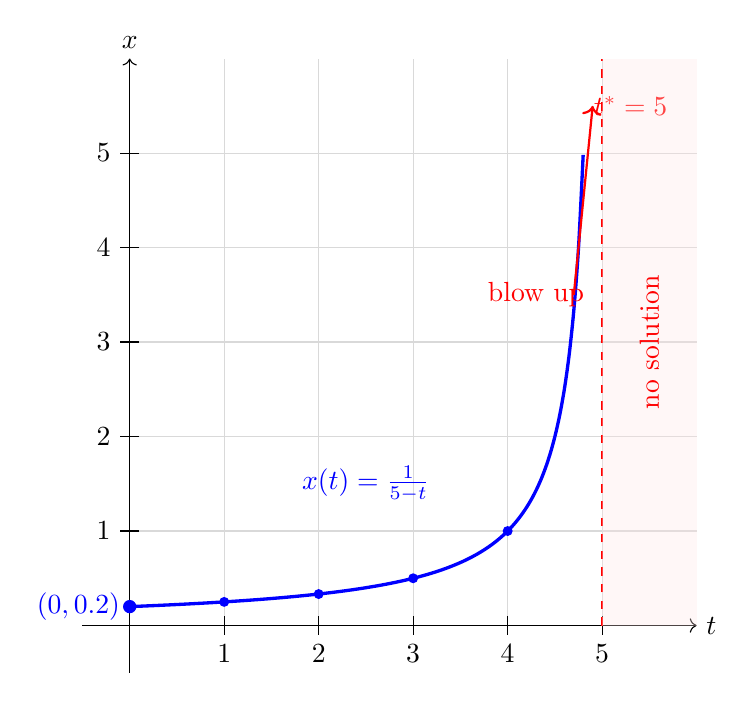
\begin{tikzpicture}[scale=1.2]
    % Axes
    \draw[->] (-0.5,0) -- (6,0) node[right] {$t$};
    \draw[->] (0,-0.5) -- (0,6) node[above] {$x$};

    % Grid
    \foreach \x in {1,2,3,4,5}
        \draw[gray!30] (\x,0) -- (\x,6);
    \foreach \y in {1,2,3,4,5}
        \draw[gray!30] (0,\y) -- (6,\y);

    % Tick marks and labels
    \foreach \x in {1,2,3,4,5}
        \draw (\x,0.1) -- (\x,-0.1) node[below] {\x};
    \foreach \y in {1,2,3,4,5}
        \draw (0.1,\y) -- (-0.1,\y) node[left] {\y};

    % Vertical asymptote at t = 5
    \draw[red, thick, dashed] (5,0) -- (5,6);
    \node[red] at (5.3, 5.5) {$t^* = 5$};

    % Solution curve x(t) = 1/(5-t)
    \draw[blue, very thick, domain=0:4.8, samples=100, smooth]
        plot (\x, {1/(5-\x)});

    % Initial point
    \fill[blue] (0, 0.2) circle (2pt);
    \node[blue, left] at (0, 0.2) {$(0, 0.2)$};

    % Some reference points
    \fill[blue] (1, 0.25) circle (1.5pt);
    \fill[blue] (2, 0.333) circle (1.5pt);
    \fill[blue] (3, 0.5) circle (1.5pt);
    \fill[blue] (4, 1.0) circle (1.5pt);

    % Arrow indicating blow up
    \draw[->, red, thick] (4.7, 3.5) -- (4.9, 5.5);
    \node[red] at (4.3, 3.5) {blow up};

    % Label the curve
    \node[blue] at (2.5, 1.5) {$x(t) = \frac{1}{5-t}$};

    % Shaded region where solution doesn't exist
    \fill[red!10, opacity=0.3] (5,0) rectangle (6,6);
    \node[red] at (5.5, 3) {\rotatebox{90}{no solution}};
\end{tikzpicture}
\end{center}

\subsection*{Step 5: Describe the Sketch Features}

\begin{itemize}[leftmargin=*]
\item \stage{STAGE X (Key features shown):}
\begin{enumerate}
    \item \textbf{Initial condition:} Point at $(0, 0.2)$
    \item \textbf{Solution curve:} Blue curve increasing from $(0, 0.2)$ toward infinity
    \item \textbf{Vertical asymptote:} Red dashed line at $t = 5$
    \item \textbf{Blow-up:} Curve approaches infinity as $t \to 5^-$
    \item \textbf{Non-existence region:} Shaded area for $t \geq 5$ where solution doesn't exist
\end{enumerate}

\item \stage{STAGE Y (Mathematical properties):}
\begin{itemize}
    \item Strictly increasing: $\dot{x} = x^2 > 0$ for all $t < 5$
    \item Concave up: $\ddot{x} = 2x^3 > 0$ for all $t < 5$
    \item Smooth: infinitely differentiable on $[0, 5)$
    \item Asymptotic: $\lim_{t \to 5^-} x(t) = +\infty$
\end{itemize}

\item \stage{STAGE Z (Physical interpretation):}
This could represent:
\begin{itemize}
    \item Population growing with quadratic birth rate
    \item Temperature in thermal runaway
    \item Concentration in autocatalytic reaction
\end{itemize}

The model predicts catastrophic growth (blow up) at $t = 5$ time units.
\end{itemize}

\subsection*{Answer to Problem 2(d)}

\begin{tcolorbox}[colback=blue!5!white,colframe=blue!75!black,title=\textbf{Solution to 2(d)}]

\textbf{Parameters:}
\begin{itemize}
    \item $a = 1$, $x_0 = 0.2$
    \item Solution: $x(t) = \frac{0.2}{1 - 0.2t} = \frac{1}{5-t}$
    \item Blow-up time: $t^* = 5$
    \item Domain: $t \in [0, 5)$
\end{itemize}

\textbf{Sketch features:}
\begin{itemize}
    \item Starts at $(0, 0.2)$
    \item Increases gradually at first, then more rapidly
    \item Becomes vertical as $t \to 5^-$
    \item Has vertical asymptote at $t = 5$ (red dashed line)
    \item No solution exists for $t \geq 5$
    \item Curve is smooth, increasing, and concave up on $[0, 5)$
\end{itemize}

\textbf{Sample values:}
\begin{itemize}
    \item $x(0) = 0.2$
    \item $x(1) = 0.25$
    \item $x(2) \approx 0.33$
    \item $x(3) = 0.5$
    \item $x(4) = 1.0$
    \item $x(4.9) = 10$
    \item $x(5^-) \to \infty$
\end{itemize}
\end{tcolorbox}

\newpage

\section*{Summary and Key Insights}

\subsection*{Complete Analysis of $\dot{x} = ax^2$}

\begin{enumerate}
\item \textbf{Existence and Uniqueness (Local):}
\begin{itemize}
    \item Solution exists and is unique near $t = 0$
    \item Guaranteed by Picard-Lindelöf theorem (local Lipschitz continuity)
\end{itemize}

\item \textbf{Explicit Solution:}
\begin{equation}
x(t) = \frac{x_0}{1 - ax_0 t}
\end{equation}

\item \textbf{Domain of Existence:}
\begin{equation}
\begin{cases}
t \in [0, \frac{1}{ax_0}) & \text{if } ax_0 > 0 \text{ (blow up in forward time)} \\
t \in (\frac{1}{ax_0}, \infty) & \text{if } ax_0 < 0 \text{ (blow up in backward time)} \\
t \in \mathbb{R} & \text{if } ax_0 = 0 \text{ (global existence)}
\end{cases}
\end{equation}

\item \textbf{Finite Time Blow Up:}
\begin{itemize}
    \item When $ax_0 > 0$: solution blows up at $t^* = \frac{1}{ax_0}$
    \item $\lim_{t \to t^*-} x(t) = +\infty$
    \item Solution does not exist for $t \geq t^*$
\end{itemize}
\end{enumerate}

\subsection*{Comparison: Local vs. Global Properties}

\begin{center}
\begin{tabular}{|l|l|l|}
\hline
\textbf{Property} & \textbf{Local} & \textbf{Global} \\
\hline
Existence & Yes (guaranteed) & No (finite time blow up) \\
Uniqueness & Yes (guaranteed) & N/A (doesn't exist globally) \\
Lipschitz continuity & Yes (locally) & No (globally) \\
Domain & Some $[0, \delta)$ & Only $[0, t^*)$ where $t^* < \infty$ \\
\hline
\end{tabular}
\end{center}

\subsection*{Physical Examples of Finite Time Blow Up}

\begin{enumerate}
\item \textbf{Population dynamics:} Super-exponential growth with $\dot{N} = rN^2$ (e.g., bacteria with perfect conditions and quadratic reproduction)

\item \textbf{Thermal runaway:} Temperature $T$ with $\dot{T} = \alpha T^2$ where reaction rate grows quadratically

\item \textbf{Financial bubbles:} Asset price with feedback: higher price attracts more buyers

\item \textbf{Social dynamics:} Viral spreading with $\dot{I} = \beta I^2$ (quadratic infection rate)
\end{enumerate}

\subsection*{Key Takeaways from Course Perspective}

\critical{MAIN LESSONS:}

\begin{enumerate}
\item \textbf{Local $\neq$ Global:} Existence and uniqueness theorems typically give local results. Global existence requires additional analysis.

\item \textbf{Lipschitz matters:} Lack of global Lipschitz continuity is a warning sign for potential finite time blow up.

\item \textbf{Nonlinearity creates complexity:} Linear ODEs ($\dot{x} = ax$) have global solutions. Nonlinear ODEs ($\dot{x} = ax^2$) can blow up.

\item \textbf{Maximal interval of existence:} Every IVP has a maximal interval of existence. For $\dot{x} = ax^2$, this is $[0, t^*)$ or $(t^*, \infty)$ depending on signs.

\item \textbf{Model breakdown:} Finite time blow up often indicates the mathematical model is no longer valid near $t^*$ (physical constraints, regime changes, etc. must be included).
\end{enumerate}

\subsection*{Connection to Future Topics}

This example illustrates fundamental concepts that appear throughout the course:
\begin{itemize}
    \item \textbf{Phase space analysis:} Understanding where solutions exist and their behavior
    \item \textbf{Equilibria and stability:} For $\dot{x} = ax^2$, only $x = 0$ is an equilibrium (unstable if $a \neq 0$)
    \item \textbf{Qualitative vs. quantitative:} We can understand blow up qualitatively even without explicit solutions
    \item \textbf{Bifurcations:} At $a = 0$, the behavior changes drastically (from blow up to global existence)
\end{itemize}

\vfill

\begin{center}
\Large\textbf{END OF QUESTION 2 SOLUTIONS}
\end{center}

\end{document}
